\documentclass{article}
\usepackage[utf8]{inputenc}

\usepackage{graphicx}
\usepackage[version=4]{mhchem}
\usepackage{siunitx}
\usepackage{glossaries}
\usepackage{xr} % For cross-referencing wit the supplemental information

\externaldocument{supplement}

% Drafting

\usepackage[latexmk]{lwarp}

\usepackage{xcolor,soul}
\usepackage{fullpage}
\usepackage{setspace}
\usepackage{blindtext}
\doublespacing

\definecolor{mwcolor}{HTML}{8af67d}
\definecolor{vgcolor}{HTML}{c88bff} % MPL purple
\definecolor{citecolor}{HTML}{c696f0} % MPL purple


% Tools for leaving todo notes around
\usepackage[colorinlistoftodos]{todonotes}
%% \renewcommand{\todo}{}
%% \renewcommand{\hl}[1]{#1}
\newcommand{\citeme}[1]{%
  \todo[color=citecolor]{%
  \ifstrempty{#1}{[citation needed]}{[cite: #1]}%
  }%
}
\newcommand{\mw}[2]{%
  \sethlcolor{mwcolor}\hl{#2}\sethlcolor{yellow}%
  \ifstrempty{#1}{}{%
    \todo[color=mwcolor]{#1 [MW]}%
  }%                  
}
\newcommand{\vg}[2]{%
  \sethlcolor{vgcolor}\hl{#2}\sethlcolor{yellow}%
  \ifstrempty{#1}{}{%
    \todo[color=vgcolor]{#1 [VG]}%
  }%                  
}

\usepackage{authblk}

\title{Origin of Rapid Delithiation In Secondary Particles Of \nca{} and \nmc{} Cathodes}

\author[1,2,3]{Mark Wolfman}
\author[1]{Brian M.\ May}
\author[4]{Vishwas Goel}
\author[4]{Sicen Du}
\author[5,6]{Young-Sang Yu}
\author[7]{Nicholas V.\ Faenza}
\author[7]{Nathalie Pereira}
\author[8]{Antonin Grenier}
\author[3]{Kamila M.\ Wiaderek}
\author[3]{Ruqing Xu}
\author[9]{Jiajun Wang}
\author[8]{Karena W.\ Chapman}
\author[7]{Glenn G. Amatucci}
\author[4]{Katsuyo Thornton}
\author[1]{Jordi Cabana\thanks{Corresponding author: jcabana@uic.edu}}

\affil[1]{Department of Chemistry, University of Illinois at Chicago}
\affil[2]{Chemical Sciences and Engineering Division, Argonne National Laboratory}
\affil[3]{X-ray Science Division, Advanced Photon Source, Argonne National Laboratory}
\affil[4]{Department of Materials Science and Engineering, University of Michigan}
\affil[5]{Department of Physics, Chungbuk National University}
\affil[6]{Advanced Light Source, Lawrence Berkeley National Laboratory}
\affil[7]{Energy Storage Research Group, Department of Materials Science and Engineering, Rutgers, The State University of New Jersey}
\affil[8]{Department of Chemistry, Stony Brook University}
\affil[9]{Harbin Institute of Technology}

\date{}

\newcommand{\nca}[1]{\ce{Li_{#1}Ni_{0.8}Co_{0.15}Al_{0.05}O_2}}
\DeclareRobustCommand{\nmc}[2][]{%
    \ifstrempty{#1}{%
        \ce{Li_{#2}Ni_{y}Mn_{z}Co_{1-y-z}O2}}{}%
    \ifstrequal{#1}{333}{%
        \ce{Li_{#2}Ni_{1/3}Mn_{1/3}Co_{1/3}O2}}{}%
    \ifstrequal{#1}{532}{%
        \ce{Li_{#2}Ni_{0.5}Mn_{0.3}Co_{0.2}O2}}{}%
}

% Techniques
\newacronym{xrd}{PXRD}{powder X-ray diffraction}
\newacronym{uxrd}{µ-XRD}{X-ray microdiffraction}
\newacronym{txm}{TXM}{transmission X-ray microscopy}
\newacronym{xas}{XAS}{X-ray absorbance spectroscopy}
\newacronym{xanes}{XANES}{X-ray absorbance near edge spectroscopy}
\newacronym{iscat}{iSCAT}{optical interferometric scattering microscopy}

% Facilities and organizations
\newacronym{ssrl}{SSRL}{Stanford Synchrotron Radiation Lightsource}

% Chemistry
%\newacronym{ecd}{ECD}{exchange current density}
\newacronym{ecd}{$i_0$}{exchange current density}
\newacronym{od}{OD}{optical depth}
\newacronym{ocv}{OCV}{open circuit voltage}

% Particles in u-XRD mapping
\newacronym{p1}{P1}{particle 1}
\newacronym{p2}{P2}{particle 2}
\newacronym{p3}{P3}{particle 3}



\begin{document}

\maketitle

%%%%%%%%%%%%%%%%%%%%%%%
\section{Introduction}
%%%%%%%%%%%%%%%%%%%%%%%

%%%%%%%%%%%%%%%%%%
\section{Results}
%%%%%%%%%%%%%%%%%%

\subsection{\Gls{uxrd} - Interparticle Dynamics}

\si{\milli\ampere\hour\per\gram}

For each particle of study, the individual 2D diffraction patterns
collected at each X-Y mapping position were integrated to 1D
patterns. The 1D patterns for each mapping position within a particle
were subsequently summed for points collected during the reaction, and
plotted in \ref{fig:xrd-echem} as a function of time. These summations
are useful to monitor the overall evolution of diffraction peaks
during oxidation and reduction of the cathode material for each
particle observed. The diffraction patterns for all three particles in
the pristine condition match well with literature for \nca{}
\cite{Robert2015a}. There was an extra feature that varies in
intensity at Q\SI{\approx3.6}{\per\angstrom}, representative of
metallic \ce{Li} (PDF \#00-001-1131). Small extraneous peaks occurred
due to random aberrations in individual pixels on the diffraction
detector.

The diffraction peaks for P1 began to shift at the onset of oxidation
(\ref{fig:xrd-echem}a). The shifts observed in P1 were consistent with
similar observations of \emph{operando} XRD of the ensemble average,
as opposed to individual particles in \nca{} electrodes, in prior work
\cite{Robert2015, Grenier2017}. P2 (\ref{fig:xrd-echem}b) also had a
change in XRD peak positions during cycling. While the peak positions
of the extreme states (pristine, charged, discharged) were consistent
with those of P1, the peaks did not begin shifting until the cell was
at a potential of \SI{\approx4.5}{\volt}. Both P1 and P2 discharged at
approximately the same rate. P3 (\ref{fig:xrd-echem}c) had no apparent
change in diffraction peak positions during charge or discharge. This
may have been due to poor connection to the carbon and binder of the
electrode.

A close inspection of the (003) and (104) diffraction peaks during
oxidation is shown in \ref{fig:ind-peaks}. The (003) reflection had an
initial decrease in $Q$, corresponding to an expansion of the $c$ axis
of the structure of the oxide, which represents the stacking of the
alternating transition metal and lithium layers. It was followed by a
sudden opposite shift beyond the initial position, indicating
shrinkage of the lattice along the same direction, while still during
delithiation. This trend has been reported before. The initial
expansion is attributed to electrostatic repulsion by the \ce{O^{2-}}
ions when \ce{Li+} ions are initially removed between consecutive
layers \cite{Robert2015}. In turn, the subsequent collapse is driven
by steric effects, and reflect the complete removal of \ce{Li+} ions,
which act as pillars of the layered framework. The (104) diffraction
peak gradually shifted to higher $Q$, or lower $d$, upon removal of
\ce{Li} from the material. It reflects the balance between the trend
along $c$ and the continuous decrease in the $a$ dimension. In this
case, the decrease reflects the shortening of metal oxygen distances
due to the oxidation of the transition metal ions (mainly \ce{Ni}),
which decreases their ionic radius.

Unit cell parameters for each diffraction pattern in
\ref{fig:xrd-echem} were extracted through Le Bail refinements and
plotted as a function of cell potential for P1 and P2
(\ref{fig:cell-pars}). The unit cell parameters reflected the trends
observed in the diffractograms presented in \ref{fig:xrd-echem}, as
well as measurements of the ensemble average of an electrode available
in the literature \cite{Robert2015a}. The cell parameters for P1
(\ref{fig:cell-pars}a-b) began shifting at a cell potential between
\SIrange{3.0}{3.8}{\volt}. The precise value is unknown as the
temporal resolution of the experiment was not high enough to capture a
full map during the rapid increase in potential at the beginning of
the charge. The unit cell parameters for P2 began shifting at
\SI{\approx4.5}{\volt}, consistent with the peak shifts in
\ref{fig:xrd-echem}b and the maps in \ref{fig:amap} and
\ref{fig:cmap}. These results led to the qualitative conclusion that
the rates of delithiation of each individual particle were different
and not uniquely represented by the electrochemical response collected
for the whole electrode.

\subsection{u-XRD - Rates of (De)lithiation}

Comparison of the XRD patterns and unit cell parameters for individual
particles during the first cycle demonstrated differences in rates of
reaction. By estimating the amount of \ce{Li} present in the material
at different points during the cathode oxidation, we can quantify the
rate of delithiation. The \ce{Li} content can be directly related to
the unit cell parameters of P1 and P2 at different points in time, by
correlating them with XRD measurements of the ensemble average of a
\nca{} electrode during galvanostatic cycling from Robert et al
\cite{Robert2015}. In this reference study, \nca{} was cycled twice
with a cutoff potential of \SI{4.8}{\volt} and the cell parameters
were associated to the average \ce{Li} content in the material
calculated from the specific capacity, or charge passed, of the cell
(i.e., Coulometrically). During the first cycle, the overall \nca{}
electrode underwent a heterogeneous transformation driven by kinetic
limitations due to the presence of \ce{Li2CO3}, which is
electronically insulating, on the particle surfaces. \ce{Li2CO3} is
oxidized to \ce{CO2} during this first oxidation. As a result, in the
second cycle, the electrode transformed via the expected pathways of
solid solution. We compared our data to the second cycle from the work
by Robert et al, since we did not see any evidence of heterogeneous
behavior in either the electrochemistry or XRD patterns of individual
particles (\ref{fig:xrd-echem}). In order to directly compare trends
in \ce{Li} content, the experimental unit cell parameters were shifted
so that the unit cell parameters for the pristine state were equal to
first value for the second charge of the reference data, which
accounts for scalar discrepancies in the measurement.

\ref{fig:rates} shows how the \ce{Li} content within \nca{} changed as
a function of time during the charge-discharge
cycle. \ref{table:rates} and \ref{table:ratesp2} show the rates of
delithiation (in terms of hours), calculated by measuring the
variation in \ce{Li} content extracted from the measured change in $c$
parameter during selected time regions for P1 and P2,
respectively. The same trends were observed with the $a$
parameter. The time regions were delineated during periods where
approximately linear changes in cell parameter were observed. In both
P1 (\ref{fig:rates}a and \ref{table:rates}) and P2 (\ref{fig:rates}b
and \ref{table:ratesp2}) the rate of delithiation started relatively
slowly, followed by a sudden increase. In the case of P1, the
delithiation during the first \SI{\approx3}{\hour} proceeded at
\SI{\approx0.025}{\ce{Li}\per\hour}, or C/40, followed by a
deceleration until \SI{\approx9}{\hour} passed. After this period, the
overall content of the particle was
\ce{Li_{0.88}Ni_{0.80}Co_{0.15}Al_{0.05}O2}. At this point, the
reaction dramatically accelerated nearly 10-fold from the initial
rate, to \SI{\approx0.3}{\ce{Li}\per\hour}, or C/3.33 until an average
composition \nca{0.53} where the rate decelerated again until the sign
of the current was reverted. In the case of P2 there was very little
delithiation for the first \SI{\approx27}{\hour} of the charge of the
cell. Delithiation proceeded down to an average content of \nca{0.92}
at \SI{\approx0.03}{\ce{Li}\per\hour}, or C/33, followed by a 20-fold
increase in rate, to \SI{\approx0.66}{\ce{Li}\per\hour}, or
C/1.5. When an average composition \nca{0.53} was again reached, the
reaction slowed down, running below 0.1 \ce{Li}/h, or C/10, for the
remainder of the oxidation. Particles relithiated rapidly during cell
discharge, with no periods of slow activity. The rapid rates of
lithiation are not reflected in \ref{table:rates} and
\ref{table:ratesp2} because too few states were captured at the
beginning of the discharge. The states that were captured (negative
values for \emph{Li removed/hour}) showed faster rates of relithiation
earlier in the discharge for both P1 and P2, reflecting the fastest
rates at intermediate contents of \ce{Li} in \nca{x}, qualitatively
consistent with the oxidation.

P1 and P2 both achieved the same level of delithiation at the end of
the charge sequence, observed in \ref{fig:rates} and by the peak
positions in \ref{fig:ind-peaks}. Since P2 did not start delithiating
until late in the charge sequence, its maximum rate of delithiation
was more than double that of P1. This observation has no precedent in
the literature for reactions involving solid solutions, where
homogeneity removes the activation barrier toward nucleation of
two-phase mechanisms. It is particularly intriguing considering that
the whole electrode was discharged at a low constant current. It can
be hypothesized that it is due to subtle variations in overpotential
between particles as a result of a different connectivity with the
electrical circuit through the carbon additive (electrons) and the
pores that contain electrolyte (ions). Particle size may have also had
an impact. Since P2 was approximately half the size of P1, the \ce{Li}
diffusion lengths out of the particle would have been shorter. Neither
of these explanations is satisfactory to predict the change in rate
for an individual particle. It is worth noting that the changes happen
at approximately similar \ce{Li} contents for both particles studied,
suggesting that the oxidation of the material changes its physical
properties, such as electronic and ionic conductivity. Follow-up
experiments are needed to evaluate this point. Both particles
relithiated to \nca{x}, where $x$ was between \numrange{0.88}{0.97}.


%%%%%%%%%%%%%%%%%%%%%
\section{Discussion}
%%%%%%%%%%%%%%%%%%%%%

%%%%%%%%%%%%%%%%%%%%%%%%%%%%%%%%
\section{Materials and Methods}
%%%%%%%%%%%%%%%%%%%%%%%%%%%%%%%%

\subsection{\gls{uxrd} Mapping}

\subsubsection{Cell Preparation}

The \nca{} composite electrode tape was cast in a dry room (dew point
of \SI{<-35}{\celsius}) using the Bellcore method
\cite{Tarascon1996}. A mixture of \nca{}, poly(vinylidene
fluoride-co-hexafluoropropylene) (PVDF-HFP, Kynar 2801, Elf Atochem),
carbon black (Super P, MMM), propylene carbonate (Aldrich), and
acetone (Aldrich) was used for the casting slurry. After casting, the
tape was allowed to dry in air, and then the propylene carbonate
plasticizer was extracted by soaking the tape in 99.8\% anhydrous
diethyl ether (Aldrich). The electrode tape had a mass composition of
\SI{20}{\percent} active material, \SI{20}{\percent} carbon additive,
and \SI{60}{\percent} binder. Prior to storage in the Ar-filled
glovebox, the tape was dried under vacuum at \SI{120}{\celsius}
overnight.

The AMPIX electrochemical cell was utilized to allow X-ray penetration
through the electrode \cite{borkiewicz2012}. Lithium metal was used as
the counter electrode and the electrolyte was composed of 1M
\ce{LiPF6} in a 1:1 mixture of ethylene carbonate:dimethyl
carbonate. Glass fiber served as the separator.

\subsubsection{Mapping}
Diffraction maps were collected at the microprobe beamline at sector
34 at the Advanced Photon Source (APS), Argonne National Laboratory
(ANL). An incoming monochromatic beam at \SI{25}{\kilo\electronvolt}
(\SI{0.4959}{\angstrom}) with a size of approximately 0.5 x
\SI{0.5}{\micro\meter} was shone through the AMPIX cell onto the
sample. The intensity of the diffracted beam was collected in
transmission geometry by a MAR165 CCD detector, with 4096 x 4096
pixels, each measuring \SI{40}{\square\micro\meter}, used in 2 x 2
binning mode.

Particle locations were determined through absorption contrast imaging
over the \ce{Ni K_\alpha} emission line at
\SI{\approx8}{\kilo\electronvolt}. Once particles were located, the
sample was moved relative to the beam using a step size of
\SI{1}{\micro\meter} and an exposure time of
\SI{10}{\second}. Two-dimensional diffraction maps were collected in
this manner continuously over the charge-discharge cycle. At each
exposure, or mapping position, a single full 2D diffraction pattern,
averaging over the depth of the material, was collected (an example is
seen in \ref{fig:2Ddiffraction}). After one map was collected for each
particle, a positive current was applied so that the charge rate would
be c/20 (in which removal of a full \ce{Li} equivalent would complete
in \SI{20}{\hour}). The cut-off potential for the cell was set for
\SI{4.8}{\volt}, to ensure a complete oxidation of the \nca{}. After
holding the cell near \SI{4.8}{\volt} for several hours, the cell was
discharged at a negative current equal in magnitude to that of the
charge. The data was collected using EPICS channel-access data
acquisition and control software.

\subsubsection{Data Analysis}
The 2D diffraction data collected by the beamline was integrated using
the FIT2D software package developed by ESRF \cite{Hammersley1996,
  Hammersley1997}. The integrated data was processed with the Scimap
analysis package \cite{Wolfman2015}, in which the determination of the
peak position yielded a set of unit cell parameters for each mapping
position, which were plotted using Python. An ensemble diffraction
pattern for each particle at each state of charge was obtained by
summing the patterns at each mapping position. These patterns
underwent batch Le Bail refinement by the TOPAS software developed by
Bruker to produce plots of unit cell as a function of charge-discharge
for each particle as a whole.


%%%%%%%%%%%%%%%%%%%%%
\section{Conclusion}
%%%%%%%%%%%%%%%%%%%%%

%%%%%%%%%%%%%%%%%%%
\section*{Figures}
%%%%%%%%%%%%%%%%%%%

\begin{figure}
  \includegraphics{figures/NCA_xrd.png}
  \caption{Operando \gls{uxrd} of \nca{} secondary particle
    agglomerates during first charge. \todo{Write a more detailed
      caption.}}
\end{figure}

\begin{figure}
  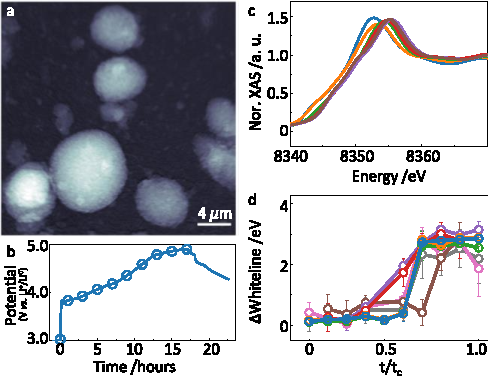
\includegraphics{figures/nca_txm.pdf}
  \caption{Operando \gls{txm} of \nca{} during first charge. (a) Mean
    optical depth frame of \nca{} particles. (b) Applied potential to
    operando cell during galvanostatic charging at \todo{what current,
      mA/g}. (c) Normalized spectra from \emph{ex-situ}
    ensemble-average \gls{xas}. (d) State-of-charge determined by
    whiteline position relative to overall state of charge in (c) for
    individual particles of \nca{}. Error bars represent one standard
    deviation over pixels within the given particle.}
\end{figure}

\begin{figure}
  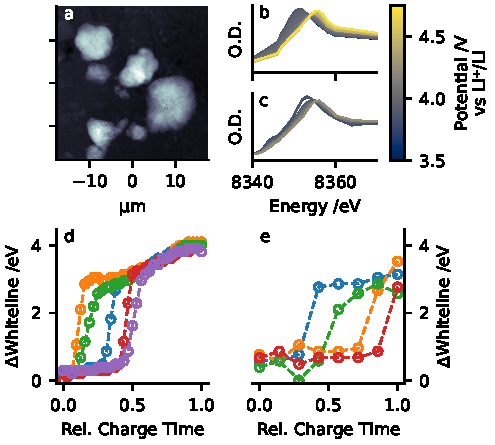
\includegraphics{figures/nmc_txm.pdf}
  \caption{Operando \gls{txm} of \nmc[333]{} and \nmc[532]{} during
    first charge. (a) Mean optical depth frame of \nmc[333]{}
    particles. (b,c) Median optical depth spectra of active material
    during charging for (b) \nmc[333]{} and (c) \nmc[532]{}. (d,e)
    Changes in median whiteline energies relative to start of charging
    cycle for individual particles of (d) \nmc[333] and (e)
    \nmc[532]{}.}
\end{figure}


\end{document}
